\section{Използвана среда и инструменти за разработка на платформата}

\FloatBarrier
\subsection{Среда за разработка на софтуера}
\FloatBarrier

Изградената среда за разработка на софтуера е конфигурируема и поддрържа базата микроконтролери от семейство \textit{STM32M4xxx}.
Като основа е използвана автоматичната система за изгращане \textit{GNU make}, която позволява насочена обработка на файловете, изграждащи софтуера и
документацията, с цел намаляване времето за обработка. \textit{GNU make} свързва всички елементи от средата и последователно изпълнява само нужните
команди с цел намаляване на използваните ресурси. Интерфейсът е команден, което позволява допълнителни нива на автоматизиране на процесите по разработка.

За компилация е използван свободният комилатор на \textit{GNU} 
\textit{GCC (GNU Comiler Collection) ARM NON-EABI (No Embedded-Application Binary Interface)}. Тази разновидност на компилатора е неспецифична към
целева операционна система, което е нужно, тъй като разработваният софтуер няма да работи под операционна система. Тази разновидност на комилатора също е
неспецифична към производителя на процесора.
\textit{GCC ARM NON-EABI} е колекция от свързани инстументи, за разработка на софтуер за системи с ядро \textit{ARM}.
Състои се от комилатор на езика C, асемблатор, линкер, инстументи за преглед и конверсия между стандартни формати двоични файлове.

За връзка с контролера е изполван командният пакет за \textit{ST-LINK} на \textit{STMicroelectronics}.
Пакетът предоставя команди за връзка с програматора \textit{ST-LINK V2}, чрез който се програмира микроконтролерът.
Пакетът се използва също за управление на порта за дебъг, през който се осъществява дебъг комуникацията.

Като дебъгер е използван свободният дебъгер на \textit{GNU}
\textit{GDB}. Той може да се използва както за локално така и за отдалечено дебъгване.
Тъй като микроконтролерът не е локален, използваме командния пакет за \textit{ST-LINK} да конфигурираме порт за дебъг,
към който се свързваме чрез \textit{GDB}.

За писането на софтуера е изполван терминалният текстов редактор \textit{VIM} поради удобния си команден интерфейс.
За генериране на всички софтуерни тагове, които \textit{VIM} ще използва за подпомагане на процеса за разработка, 
е използван софтуерът \textit{ctags}, който обработва релевантните файлове и поддържа опростена база данни за всички индентификатори,
имена и тагове, които \textit{VIM} изпозва спрямо контекста.

Основата за средата за разработка съм публикувал в публично хранилище на GitHub \cite{github_stm32_base}.

\FloatBarrier


\subsection{Инструменти}

За хардуерната част са използвани стандартни инструменти, като отвертки, шестограми, винтоверт, нивелир, макетен нож, рулетка, шублер, трион, шкурка, поялник, пистолет за топъл силикон и т.н.


\subsubsection{Логически анализатор и генератор на (дигитални) сигнали}
\FloatBarrier
Тъй-като този труд  има за цел управление и работа с хардуер и 
създаване на хардуерни драйвери, е нужен начин за анализ и диагностика на крайната комуникация.
Затова е избран модулът \textit{SQ50 - logic analyzer } от семейство \textit{SQ series (ScanaQuad)} на  \textit{IKALOGIC S.A.S.} (\autoref{fig:logic_analyzer_hardware}).
Модулът разполага с \(4\) канала с възможност за използване за вход и/или изход,
максималана честота на дискретизация \(50MHz\),
максимална честота на измерим/генерируем дигитален сигнал \(12MHz\), 
входно напрежение \(\pm 5V\),
входен импеданс \(1M\Omega/4pF\),
kонфигурируем изходен драйвър (Push-Pull/open-drain),
и максималнен изходен ток \(20mA\) \cite{manual_sq50}.

\begin{figure}[hbpt!]
    \centering
    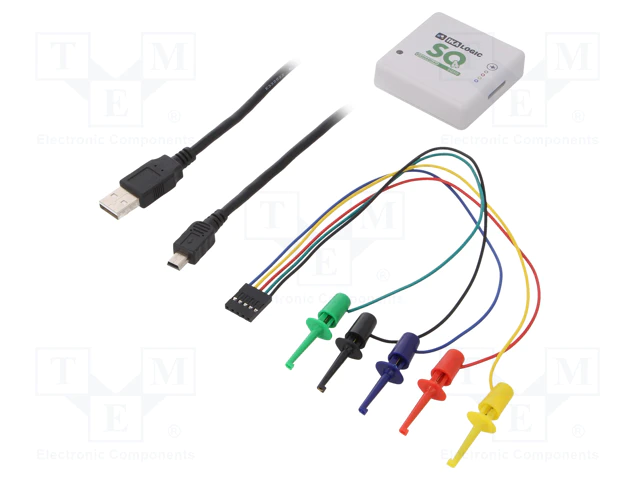
\includegraphics[width=0.5\textwidth]{SQ50-logic-analyzer}
    \caption{Логически анализатор SQ50}
    \label{fig:logic_analyzer_hardware}
\end{figure}


\FloatBarrier

\textit{SQ50 - logic analyzer } е използван със софтуерният продукт \textit{ScanaStudio} (\autoref{fig:scana_studio_window}) на \textit{IKALOGIC S.A.S.}.
\textit{ScanaStudio} е достъпен за платформите \textit{Windows 7, 8 и 10}, \textit{LINUX UBUNTU 16.04 и по-нови (x64)}, \textit{MACOS 10.9 и по-нови}.
Софтуерният продукт позволява възможности за конфигурация на хардуера от семейство \textit{SQ series (ScanaQuad)}, както и четене, експорт и представяне на
данните, постъпили от модула.
Към продукта \textit{IKALOGIC S.A.S.} предоставят набор от готови разширения, 
които са свободно достъпни и позволяват:
параметрично генериране на основни типове сигнали (ШИМ, честотна модулация, I2C),
декодиране за сигнали (USART, I2C, I2S, SPI, PWM, SWD, 1-Wire и т.н.),
конфигурируем източник на задействане (trigger) при определени условия -- получена специфична последователност, логическа промяна, специфичен/случаен валиден кадър от комуникационен протокол и т.н.


\begin{figure}[htpb!]
    \centering
    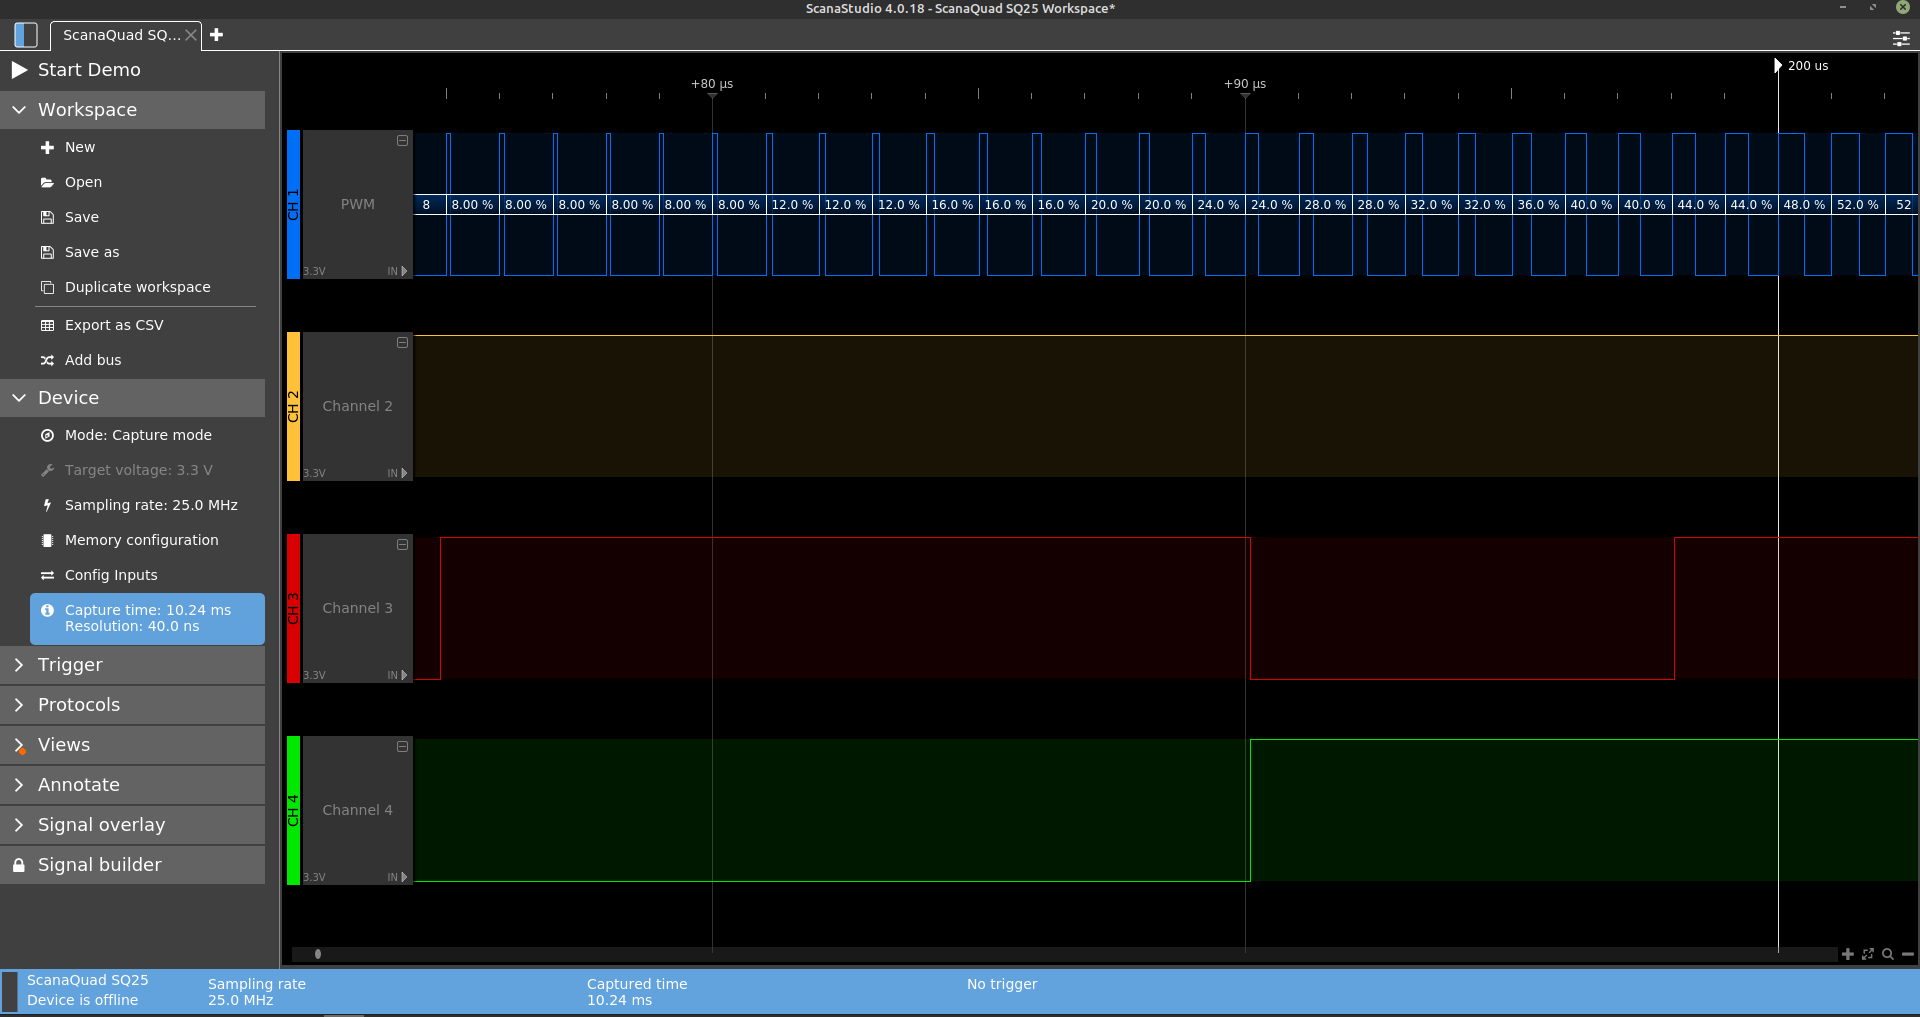
\includegraphics[width=0.9\textwidth]{scana_studio_window}
    \caption{Прозорец Scana Studio}
    \label{fig:scana_studio_window}
\end{figure}

\FloatBarrier


\subsubsection{Балансьор за витла}
\FloatBarrier


Използван е балансьор за витла (\autoref{fig:prop_balancer}) с цел балансиране на витлата.
Баланьорът сам по себе си е тънка прецизно изработена права ос с тънка резба, в комбинация с две прецизно изработени конични гайки с успоредна на оста задна част,
за да фиксират витлото успоредно спрямо оста, както и да центрират средата на отвора.
 
\begin{figure}[htpb!]
    \centering
    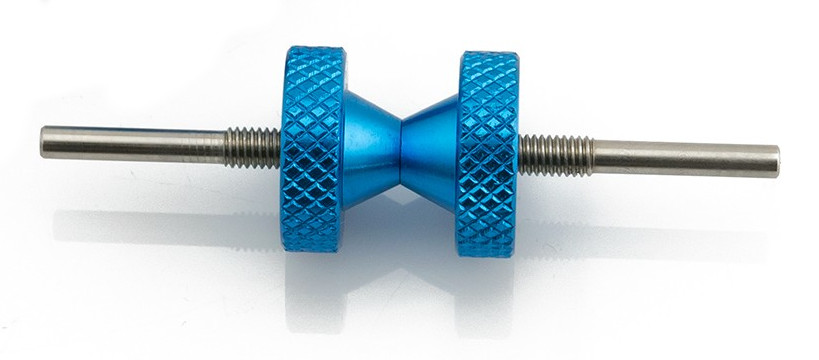
\includegraphics[width=0.8\textwidth]{prop_balancer}
    \caption{Балансьор за витла}
    \label{fig:prop_balancer}
\end{figure}




\subsubsection{UART към USB конвертор}
\FloatBarrier


Използван е конвертор USART към USB, за приемане на данните от контролера и записваненето им
на Linux системата, за допълнителна обработка и генериране на фигури.

\begin{figure}[htpb!]
    \centering
    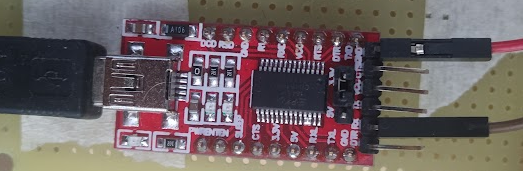
\includegraphics[width=0.8\textwidth]{uart_usb}
    \caption{UART към USB конвертор}
    \label{fig:prop_balancer2}
\end{figure}


\subsubsection{3D Принтер}
\FloatBarrier

За изработване на платформата е използван 3D принтера \textit{Ender 3 V2} (\autoref{fig:3d_printer_hardware} ) на \textit{Creality}.
Неговата технология на работа е FFF (Fused Fillament Fabrication -- производство чрез стопени нишки), която е форма на адитивно производство.
Принтерът е оборудван с \(0.4mm\) дюза,
легло със загравяне и стъклена повърхност
и има работен обем \(220x220x250mm\), 
и диаметър на нишката \(1.75mm\) \cite{user_manual_3d_printer}.

За целите на този труд е използвана нишка от ECO PLA (рециклирана полимлечна киселина), произведена от \textit{3D Jake} 
с диаметър \(1.75mm\),
температура на принтиране \(195\to215^{\circ}C\), 
максимална работна температура \(60^{\circ}C\),
якост на опън \(70MPa)\)
и деформация при опън \(5\%\) \cite{datasheet_ecopla}.

\begin{figure}[htpb!]
    \centering
    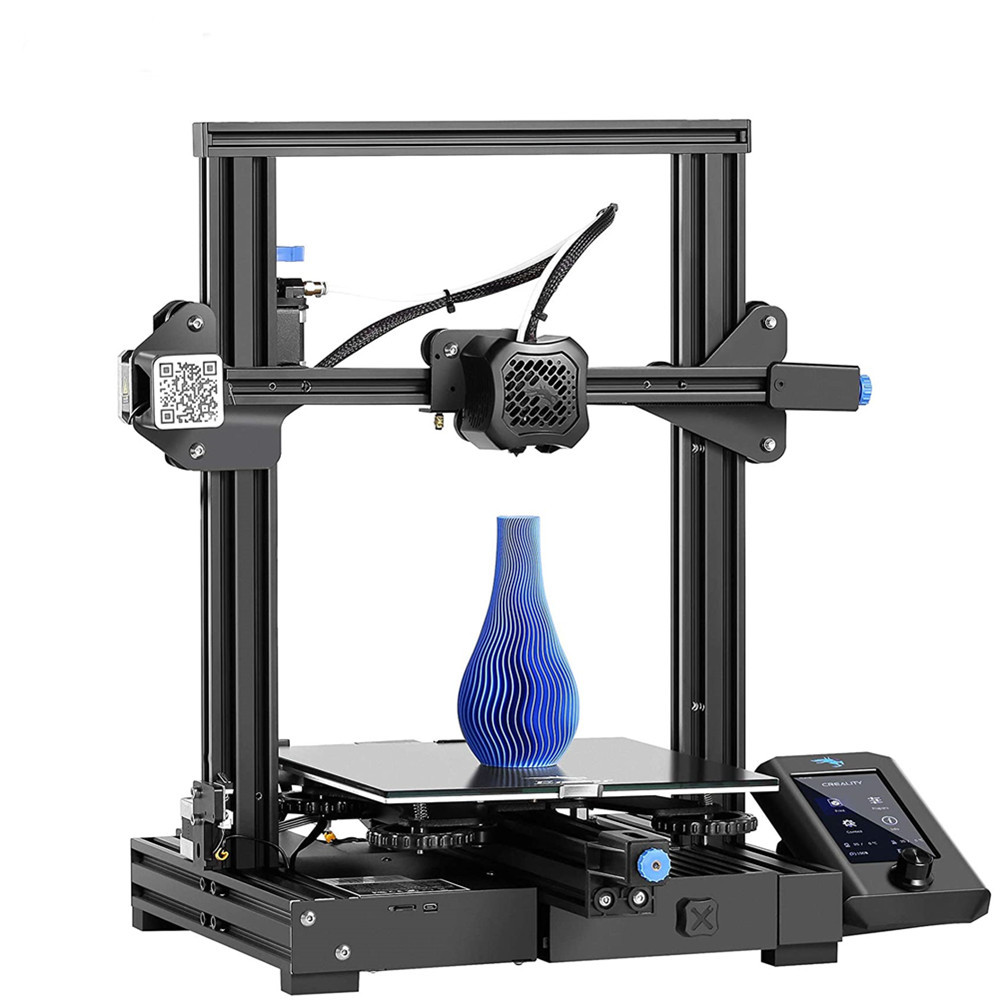
\includegraphics[width=0.7\textwidth]{3d_printer_hardware}
    \caption{3D принтер Creality Ender 3 V2}
    \label{fig:3d_printer_hardware}
\end{figure}

\FloatBarrier
За генериране на G-code, който ще бъде изпълнен от принтера, е използван софтуерният продукт
\textit{Ultimaker Cura} (\autoref{fig:ultimaker_cura_window}) на \textit{Ultimaker}.
Продуктът е конфигуриран ръчно за устройството \textit{Ender 3 V2}, тъй като не бе налично
в базата данни с готови конфигурации. 
Софтуерът позволява \enquote{нарязване} на триизмерни обекти на слоеве и конвертирането им в G-code програма за изпълнение от
устройството, както и конфигуриране на множество параметри относно процеса на принтиране.

\begin{figure}[htpb!]
    \centering
    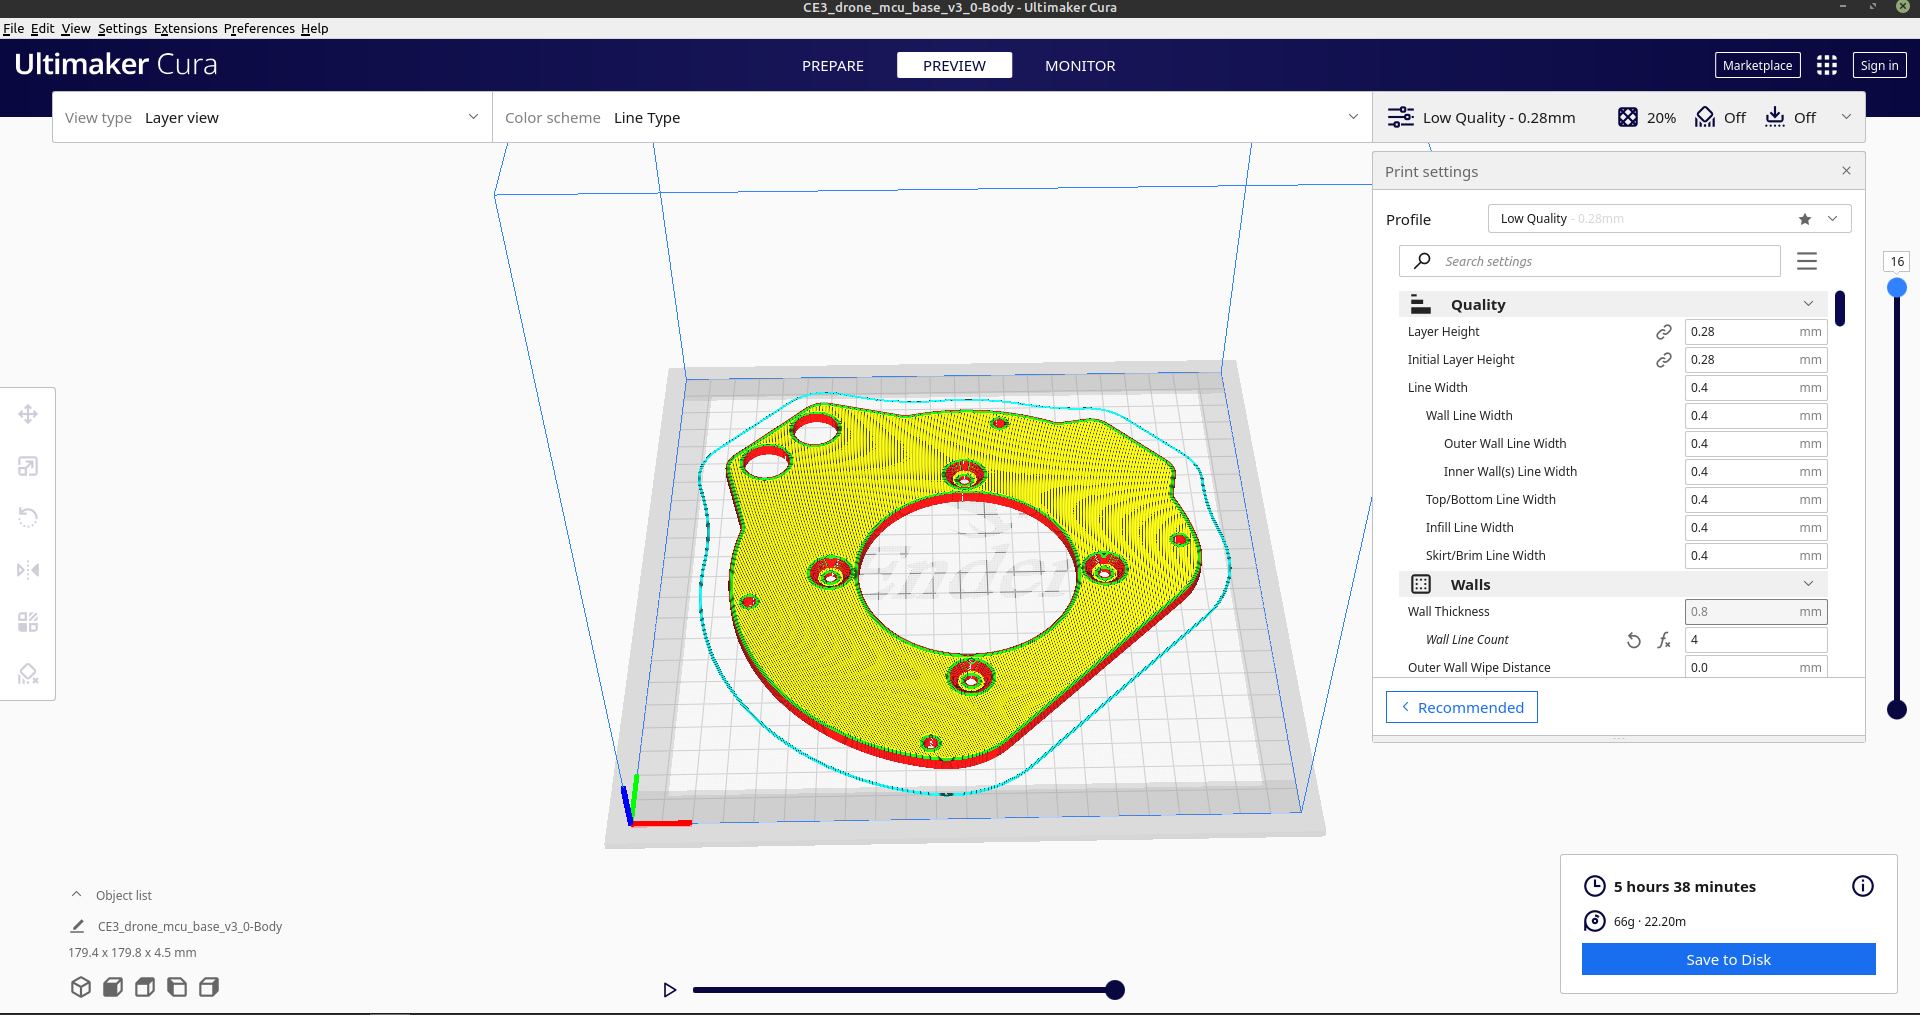
\includegraphics[width=0.9\textwidth]{ultimaker_cura_window}
    \caption{Прозорец на Ultimaker Cura}
    \label{fig:ultimaker_cura_window}
\end{figure}
\FloatBarrier
За създаване на 3D модел е използван софтуерният продукт \textit{FreeCad} \autoref{fig:freecad_window},
тъй като работи под \textit{Linux} платформа и е добре документиран, свободен и безплатен софтуер.

\begin{figure}[htpb!]
    \centering
    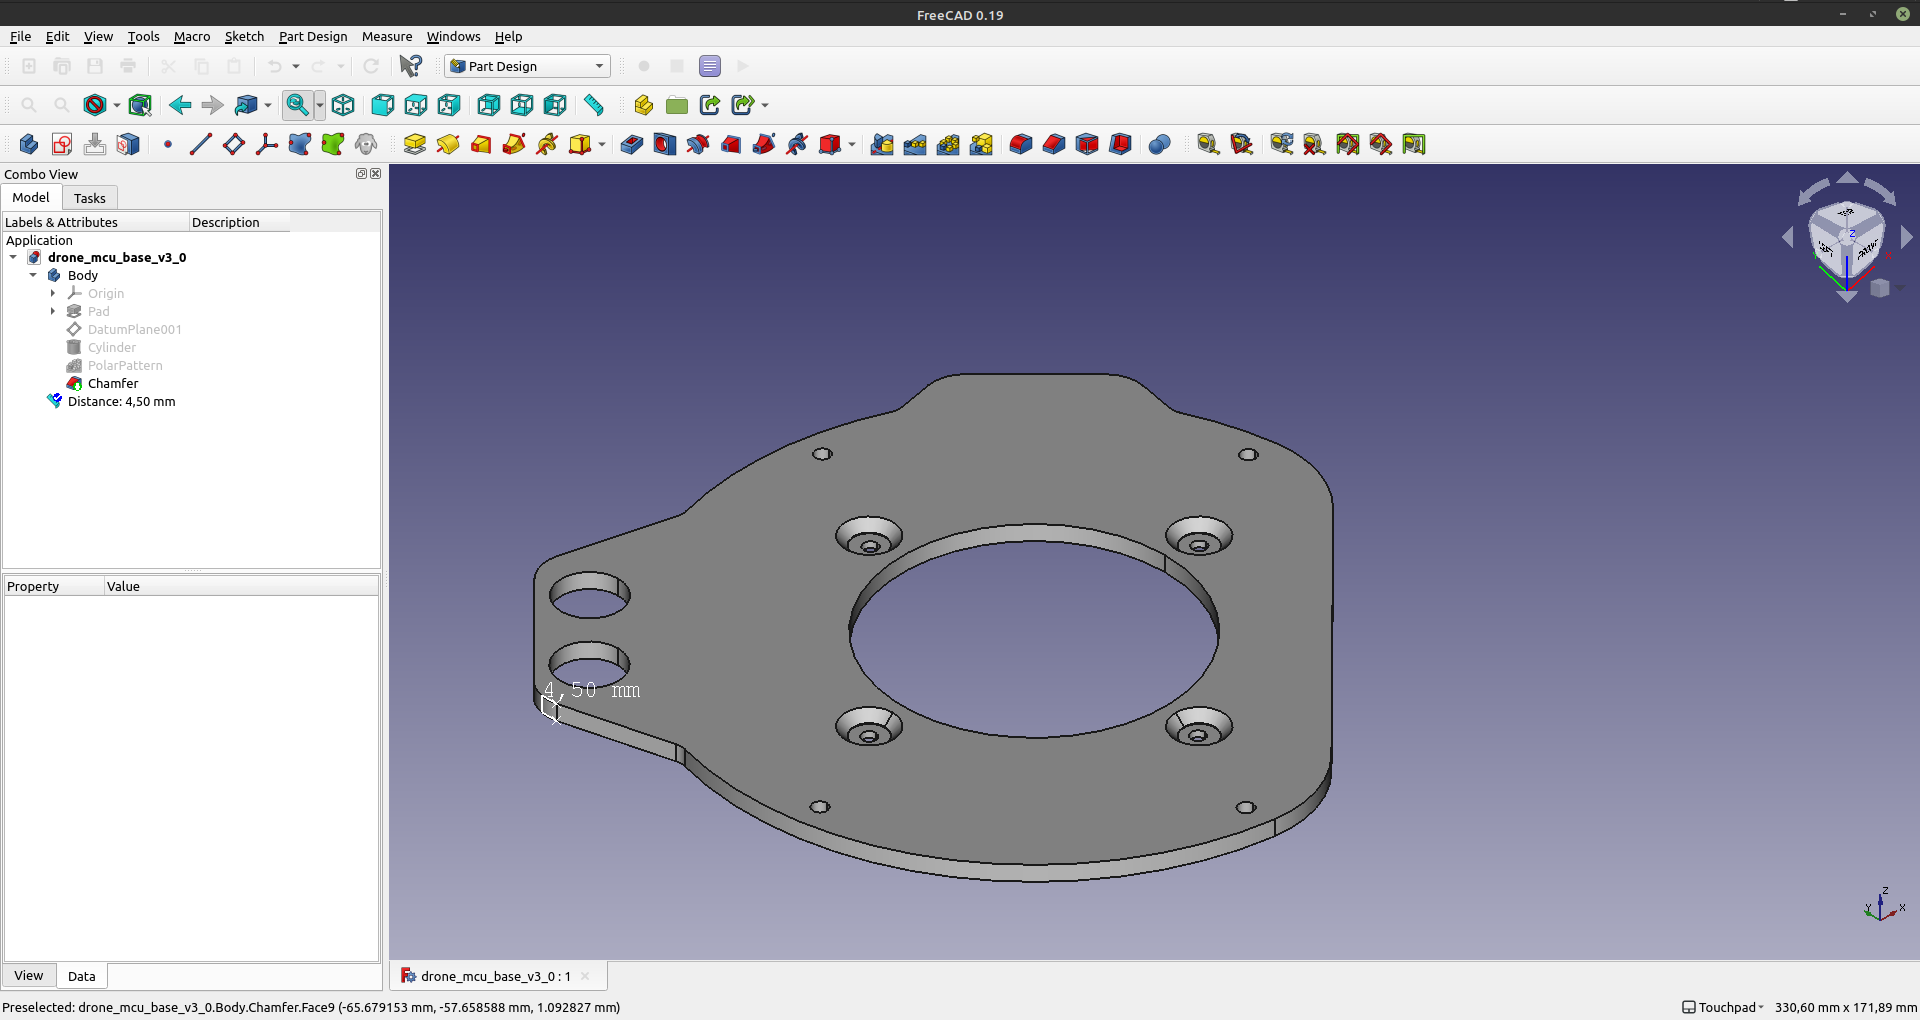
\includegraphics[width=0.9\textwidth]{freecad_window}
    \caption{Прозорец на FreeCad}
    \label{fig:freecad_window}
\end{figure}

\FloatBarrier




